\documentclass[journal,12pt,onecolumn]{IEEEtran}
\usepackage{cite}
\usepackage{graphicx}
\usepackage{amsmath,amssymb,amsfonts,amsthm}
\usepackage{algorithmic}
\usepackage{graphicx}
\usepackage{textcomp}
\usepackage{xcolor}
\usepackage{txfonts}
\usepackage{listings}
\usepackage{enumitem}
\usepackage{mathtools}
\usepackage{gensymb}
\usepackage{comment}
\usepackage[breaklinks=true]{hyperref}
\usepackage{tkz-euclide} 
\usepackage{listings}
\usepackage{gvv}                                        
%\def\inputGnumericTable{}                                 
\usepackage[utf8]{inputenc} 
\usetikzlibrary{arrows.meta, positioning}
\usepackage{xparse}
\usepackage{color}                                            
\usepackage{array}                                            
\usepackage{longtable}                                       
\usepackage{calc}                                             
\usepackage{multirow}
\usepackage{multicol}
\usepackage{hhline}                                           
\usepackage{ifthen}                                           
\usepackage{lscape}
\usepackage{tabularx}
\usepackage{array}
\usepackage{float}
\newtheorem{theorem}{Theorem}[section]
\newtheorem{problem}{Problem}
\newtheorem{proposition}{Proposition}[section]
\newtheorem{lemma}{Lemma}[section]
\newtheorem{corollary}[theorem]{Corollary}
\newtheorem{example}{Example}[section]
\newtheorem{definition}[problem]{Definition}
\newcommand{\BEQA}{\begin{eqnarray}}
\newcommand{\EEQA}{\end{eqnarray}}
\usepackage{float}
%\newcommand{\define}{\stackrel{\triangle}{=}}
\theoremstyle{remark}
\usepackage{circuitikz}
\usepackage{tikz}
\title{GATE MA 2017}
\author{EE25BTECH11030-AVANEESH}

\begin{document}
\maketitle
\begin{enumerate}

%1
\item
Consider the vector space $V = \{a_0 + a_1x + a_2x^2 : a_i \in \mathbb{R} \text{ for } i=0,1,2\}$ of polynomials of degree at most 2. Let $f: V \to \mathbb{R}$ be a linear functional such that $f(1+x)=0$, $f(1-x^2)=0$ and $f(x^2-x)=2$. Then $f(1+x+x^2)$ equals \rule{1.5cm}{0.4pt}.
\hfill (GATE MA 2017)

%2
\item
Let A be a $7 \times 7$ matrix such that $2A^2 - A^4 = I$, where I is the identity matrix. If A has two distinct eigenvalues and each eigenvalue has geometric multiplicity 3, then the total number of nonzero entries in the Jordan canonical form of A equals \rule{1.5cm}{0.4pt}.
\hfill (GATE MA 2017)

%3
\item
Let $f(z) = (x^2+y^2) + i2xy$ and $g(z) = 2xy + i(y^2-x^2)$ for $z=x+iy \in \mathbb{C}$. Then, in the complex plane $\mathbb{C}$.
\begin{enumerate}
\item f is analytic and g is NOT analytic
\item f is NOT analytic and g is analytic
\item neither f nor g is analytic
\item both f and g are analytic
\end{enumerate}
\hfill (GATE MA 2017)

%4
\item
If $\sum_{n=-\infty}^{\infty} a_n(z-2)^n$ is the Laurent series of the function $f(z) = \frac{z^4+z^3+z^2}{(z-2)^3}$ for $z \in \mathbb{C} \setminus {2}$, then $a_{-2}$ equals \rule{1.5cm}{0.4pt}.
\hfill (GATE MA 2017)
%5
\item
Let $f_n: \to \mathbb{R}$ be given by $f_n(x) = \frac{2x^2}{x^2 + (1-2nx)^2}$, $n=1,2,\dots$. Then the sequence $(f_n)$
\begin{enumerate}
\item converges uniformly on
\item does NOT converge uniformly on but has a subsequence that converges uniformly on
\item does NOT converge pointwise on
\item converges pointwise on but does NOT have a subsequence that converges uniformly on
\end{enumerate}
\hfill (GATE MA 2017)
%6
\item
Let $C: x^2+y^2=9$ be the circle in $\mathbb{R}^2$ oriented positively. Then $\frac{1}{\pi} \oint_C (3y - e^{\cos x^2})dx + (7x + \sqrt{y^4+11})dy$ equals \rule{1.5cm}{0.4pt}.
\hfill (GATE MA 2017)
%7
\item
Consider the following statements:
\begin{itemize}
\item[(P):] There exists an unbounded subset of $\mathbb{R}$ whose Lebesgue measure is equal to 5.
\item[(Q):] If $f:\mathbb{R} \to \mathbb{R}$ is continuous and $g:\mathbb{R} \to \mathbb{R}$ is such that $f=g$ almost everywhere on $\mathbb{R}$, then g must be continuous almost everywhere on $\mathbb{R}$.
\end{itemize}
Which of the above statements hold TRUE?
\begin{enumerate}
\begin{multicols}{2}
\item Both P and Q
\item Only P
\item Only Q
\item Neither P nor Q
\end{multicols}
\end{enumerate}
\hfill (GATE MA 2017)
%8
\item
If $x^3y^2$ is an integrating factor of $(6y^2 + axy)dx + (6xy + bx^2)dy = 0$ where $a, b \in \mathbb{R}$, then
\begin{enumerate}
\begin{multicols}{2}
\item $3a - 5b = 0$
\item $2a - b = 0$
\item $3a + 5b = 0$
\item $2a + b = 0$
\end{multicols}
\end{enumerate}
\hfill (GATE MA 2017)
%9
\item
If $x(t)$ and $y(t)$ are the solutions of the system $\frac{dx}{dt} = y$ and $\frac{dy}{dt} = -x$ with the initial conditions $x(0)=1$ and $y(0)=1$, then $x(\pi/2) + y(\pi/2)$ equals \rule{1.5cm}{0.4pt}.
\hfill (GATE MA 2017)
%10
\item
If $y = 3e^{2x} + e^{-2x} - \alpha x$ is the solution of the initial value problem $\frac{d^2y}{dx^2} + \beta y = 4\alpha x$, $y(0)=4$ and $\frac{dy}{dx}(0)=1$, where $\alpha, \beta \in \mathbb{R}$, then
\begin{enumerate}
\begin{multicols}{2}
\item $\alpha=3$ and $\beta=4$
\item $\alpha=1$ and $\beta=2$
\item $\alpha=3$ and $\beta=-4$
\item $\alpha=1$ and $\beta=-2$
\end{multicols}
\end{enumerate}
\hfill (GATE MA 2017)
%11
\item
Let G be a non-abelian group of order 125. Then the total number of elements in $Z(G) = \{x \in G : gx=xg \text{ for all } g \in G\}$ equals \rule{1.5cm}{0.4pt}.
\hfill (GATE MA 2017)
%12
\item
Let $F_1$ and $F_2$ be subfields of a finite field F consisting of $2^9$ and $2^6$ elements, respectively. Then the total number of elements in $F_1 \cap F_2$ equals \rule{1.5cm}{0.4pt}.
\hfill (GATE MA 2017)
%13
\item
Consider the normed linear space $\mathbb{R}^2$ equipped with the norm given by $|(x,y)| = |x|+|y|$ and the subspace $X = {(x,y) \in \mathbb{R}^2 : x=y}$. Let f be the linear functional on X given by $f(x,y)=3x$. If $g(x,y)=\alpha x + \beta y$, $\alpha, \beta \in \mathbb{R}$, is a Hahn-Banach extension of f on $\mathbb{R}^2$, then $\alpha - \beta$ equals \\ \rule{1.5cm}{0.4pt}.
\hfill (GATE MA 2017)
%14
\item
For $n \in \mathbb{Z}$, define $c_n = \frac{1}{\sqrt{2\pi}} \int_{-\pi}^{\pi} e^{i(n-i)x} dx$, where $i^2 = -1$. Then $\sum_{n \in \mathbb{Z}} |c_n|^2$ equals
\begin{enumerate}
\begin{multicols}{4}
\item $\cosh(\pi)$
\item $\sinh(\pi)$
\item $\cosh(2\pi)$
\item $\sinh(2\pi)$
\end{multicols}
\end{enumerate}
\hfill (GATE MA 2017)
%15
\item
If the fourth order divided difference of $f(x) = \alpha x^4 + 5x^3 + 3x + 2$, $\alpha \in \mathbb{R}$, at the points 0.1, 0.2, 0.3, 0.4, 0.5 is 5, then $\alpha$ equals \rule{1.5cm}{0.4pt}.
\hfill (GATE MA 2017)
%16
\item
If the quadrature rule $\int_0^2 f(x) dx \approx c_1 f(0) + 3f(c_2)$, where $c_1, c_2 \in \mathbb{R}$, is exact for all polynomials of degree $\le 1$, then $c_1 + 3c_2$ equals \rule{1.5cm}{0.4pt}.
\hfill (GATE MA 2017)
%17
\item
If $u(x,y) = 1+x+y+f(xy)$, where $f: \mathbb{R}^2 \to \mathbb{R}$ is a differentiable function, then u satisfies
\begin{enumerate}
\begin{multicols}{2}
\item $x\frac{\partial u}{\partial x} - y\frac{\partial u}{\partial y} = x^2 - y^2$
\item $x\frac{\partial u}{\partial x} - y\frac{\partial u}{\partial y} = 0$
\item $x\frac{\partial u}{\partial x} - y\frac{\partial u}{\partial y} = x - y$
\item $y\frac{\partial u}{\partial x} - x\frac{\partial u}{\partial y} = x - y$
\end{multicols}
\end{enumerate}
\hfill (GATE MA 2017)
%18
\item
The partial differential equation $x\frac{\partial^2 u}{\partial x^2} + (x-y)\frac{\partial^2 u}{\partial x \partial y} - y\frac{\partial^2 u}{\partial y^2} + \frac{1}{4}\left(\frac{\partial u}{\partial y} - \frac{\partial u}{\partial x}\right) = 0$ is
\begin{enumerate}
\begin{multicols}{2}
\item hyperbolic along the line $x+y=0$
\item elliptic along the line $x-y=0$
\item elliptic along the line $x+y=0$
\item parabolic along the line $x+y=0$
\end{multicols}
\end{enumerate}
\hfill (GATE MA 2017)
%19
\item
Let X and Y be topological spaces and let $f: X \to Y$ be a continuous surjective function. Which one of the following statements is TRUE?
\begin{enumerate}
\item If X is separable, then Y is separable
\item If X is first countable, then Y is first countable
\item If X is Hausdorff, then Y is Hausdorff
\item If X is regular, then Y is regular
\end{enumerate}
\hfill (GATE MA 2017)
%20
\item
Consider the topology $\mathcal{T} = {U \subseteq \mathbb{Z} : \mathbb{Z} \setminus U \text{ is finite or } 0 \notin U}$ on $\mathbb{Z}$. Then, the topological space $(\mathbb{Z}, \mathcal{T})$ is
\begin{enumerate}
\begin{multicols}{2}
\item compact but NOT connected
\item connected but NOT compact
\item both compact and connected
\item neither compact nor connected
\end{multicols}
\end{enumerate}
\hfill (GATE MA 2017)
%21
\item
Let $F(x)$ be the distribution function of a random variable X. Consider the functions:
\begin{itemize}
\item[] $G_1(x) = (F(x))^2$, $x \in \mathbb{R}$,
\item[] $G_2(x) = 1 - (1-F(x))^2$, $x \in \mathbb{R}$.
\end{itemize}
Which of the above functions are distribution functions?
\begin{enumerate}
\begin{multicols}{2}
\item Neither $G_1$ nor $G_2$
\item Only $G_1$
\item Only $G_2$
\item Both $G_1$ and $G_2$
\end{multicols}
\end{enumerate}
\hfill (GATE MA 2017)
%22
\item
Let $X_1, X_2, \dots, X_n (n \ge 2)$ be independent and identically distributed random variables with finite variance $\sigma^2$ and let $\bar{X} = \frac{1}{n} \sum_{i=1}^n X_i$. Then the covariance between $\bar{X}$ and $X_1 - \bar{X}$ is
\begin{enumerate}
\begin{multicols}{4}
\item 0
\item $-\sigma^2$
\item $-\frac{\sigma^2}{n}$
\item $\frac{\sigma^2}{n}$
\end{multicols}
\end{enumerate}
\hfill (GATE MA 2017)
%23
\item
Let $X_1, X_2, \dots, X_n (n \ge 2)$ be a random sample from a $N(\mu, \sigma^2)$ population, where $\sigma^2 = 144$. The smallest n such that the length of the shortest $95\%$ confidence interval for $\mu$ will not exceed $10$ is \rule{1.5cm}{0.4pt}.
\hfill (GATE MA 2017)
%24
\item
Consider the linear programming problem (LPP):
Maximize $4x_1 + 6x_2$
Subject to
$x_1 + x_2 \le 8$
$2x_1 + 3x_2 \ge 18$
$x_1 \ge 6$
$x_2$ is unrestricted in sign.
Then the LPP has
\begin{enumerate}
\item no optimal solution
\item only one basic feasible solution and that is optimal
\item more than one basic feasible solution and a unique optimal solution
\item infinitely many optimal solutions
\end{enumerate}
\hfill (GATE MA 2017)
%25
\item
For a linear programming problem (LPP) and its dual, which one of the following is NOT TRUE?
\begin{enumerate}
\item The dual of the dual is primal
\item If the primal LPP has an unbounded objective function, then the dual LPP is infeasible
\item If the primal LPP is infeasible, then the dual LPP must have unbounded objective function
\item If the primal LPP has a finite optimal solution, then the dual LPP also has a finite optimal solution
\end{enumerate}
\hfill (GATE MA 2017)
%26
\item
If U and V are the null spaces of $\myvec {1 & 1 & 0 & 0 \ 0 & 0 & 1 & 1 \ }$ and $\myvec{ 1 & 2 & 3 & 2 \ 0 & 1 & 2 & 1 \ }$, respectively, then the dimension of the subspace $U+V$ equals \rule{1.5cm}{0.4pt}.
\hfill (GATE MA 2017)
%27
\item
Given two $n \times n$ matrices A and B with entries in $\mathbb{C}$, consider the following statements:
\begin{itemize}
\item[(P):] If A and B have the same minimal polynomial, then A is similar to B.
\item[(Q):] If A has n distinct eigenvalues, then there exists $u \in \mathbb{C}^n$ such that $u, Au, \dots, A^{n-1}u$ are linearly independent.
\end{itemize}
Which of the above statements hold TRUE?
\begin{enumerate}
\begin{multicols}{2}
\item Both P and Q
\item Only P
\item Only Q
\item Neither P nor Q
\end{multicols}
\end{enumerate}
\hfill (GATE MA 2017)
%28
\item
Let $A=(a_{ij})$ be a $10 \times 10$ matrix such that $a_{ij}=1$ for $i \ne j$ and $a_{ii}=\alpha+1$, where $\alpha > 0$. Let $\lambda$ and $\mu$ be the largest and the smallest eigenvalues of A, respectively. If $\lambda + \mu = 24$, then $\alpha$ equals\\ \rule{1.5cm}{0.4pt}.
\hfill (GATE MA 2017)
%29
\item
Let C be the simple, positively oriented circle of radius 2 centered at the origin in the complex plane. Then $\frac{2}{\pi i} \int_C \brak{ ze^{1/z} + \tan\brak{\frac{z}{2}} + \frac{1}{(z-1)(z-3)^2} } dz$ equals \rule{1.5cm}{0.4pt}.
\hfill (GATE MA 2017)
%30
\item
Let $Re(z)$ and $Im(z)$ respectively, denote the real part and the imaginary part of a complex number z. Let $T: \mathbb{C} \cup {\infty} \to \mathbb{C} \cup {\infty}$ be the bilinear transformation such that $T(6)=0$, $T(3-3i)=i$ and $T(0)=\infty$. Then, the image of $D = {z \in \mathbb{C} : |z-3|<3}$ under the mapping $w=T(z)$ is
\begin{enumerate}
\begin{multicols}{2}
\item ${w \in \mathbb{C} : Im(w) < 0}$
\item ${w \in \mathbb{C} : Re(w) < 0}$
\item ${w \in \mathbb{C} : Im(w) > 0}$
\item ${w \in \mathbb{C} : Re(w) > 0}$
\end{multicols}
\end{enumerate}
\hfill (GATE MA 2017)
%31
\item
Let $(x_n)$ and $(y_n)$ be two sequences in a complete metric space $(X,d)$ such that $d(x_n, x_{n+1}) \le \frac{1}{n^2}$ and $d(y_n, y_{n+1}) \le \frac{1}{n}$ for all $n \in \mathbb{N}$. Then
\begin{enumerate}
\item both $(x_n)$ and $(y_n)$ converge
\item $(x_n)$ converges but $(y_n)$ need NOT converge
\item $(y_n)$ converges but $(x_n)$ need NOT converge
\item neither $(x_n)$ nor $(y_n)$ converges
\end{enumerate}
\hfill (GATE MA 2017)
%32
\item
Let $f: \to \mathbb{R}$ be given by $f(x)=0$ if x is rational, and if x is irrational then $f(x)=9^n$, where n is the number of zeroes immediately after the decimal point in the decimal representation of x. Then the Lebesgue integral $\int_0^1 f(x) dx$ equals \rule{1.5cm}{0.4pt}.
\hfill (GATE MA 2017)
%33
\item
Let $f: \mathbb{R}^2 \to \mathbb{R}$ be defined by $f(x,y) =
\begin{cases}
\sin(\frac{y^2}{x}) \sqrt{x^2+y^2}, & x \neq 0 \\
0, & x=0
\end{cases}$.
Then, at $(0,0)$,
\begin{enumerate}
\item $f$ is continuous and the directional derivative of $f$ does NOT exist in some direction
\item $f$ is NOT continuous and the directional derivatives of $f$ exist in all directions
\item $f$ is NOT differentiable and the directional derivatives of $f$ exist in all directions
\item $f$ is differentiable
\end{enumerate}
\hfill (GATE MA 2017)
%34
\item
Let D be the region in $\mathbb{R}^2$ bounded by the parabola $y^2=2x$ and the line $y=x$. Then $\iint_D 3xy ,dx,dy$ equals \rule{1.5cm}{0.4pt}.
\hfill (GATE MA 2017)
%35
\item
Let $y_1(x) = x^3$ and $y_2(x) = x^2|x|$ for $x \in \mathbb{R}$. Consider the following statements:
\begin{itemize}
\item[(P):] $y_1(x)$ and $y_2(x)$ are linearly independent solutions of $x^2\frac{d^2y}{dx^2} - 4x\frac{dy}{dx} + 6y = 0$ on $\mathbb{R}$.
\item[(Q):] The Wronskian $W(y_1, y_2)(x) = y_1(x)\frac{dy_2}{dx}(x) - y_2(x)\frac{dy_1}{dx}(x) = 0$ for all $x \in \mathbb{R}$.
\end{itemize}
Which of the above statements hold TRUE?
\begin{enumerate}
\begin{multicols}{2}
\item Both P and Q
\item Only P
\item Only Q
\item Neither P nor Q
\end{multicols}
\end{enumerate}
\hfill (GATE MA 2017)
%36
\item
Let $\alpha$ and $\beta$ with $\alpha > \beta$ be the roots of the indicial equation of $x^2 \frac{d^2y}{dx^2} - (x+1) \frac{dy}{dx} + y = 0$ at $x=0$. Then $\alpha - 4\beta$ equals \rule{1.5cm}{0.4pt}.
\hfill (GATE MA 2017)
%37
\item
Let $S_9$ be the group of all permutations of the set ${1, 2, 3, 4, 5, 6, 7, 8, 9}$. Then the total number of elements of $S_9$ that commute with $\tau = (1 \ 2 \ 3)(4 \ 5 \ 6 \ 7)$ in $S_9$ equals \rule{1.5cm}{0.4pt}.
\hfill (GATE MA 2017)
%38
\item
Let $\mathbb{Q}[x]$ be the ring of polynomials over $\mathbb{Q}$. Then the total number of maximal ideals in the quotient ring $\mathbb{Q}[x]/\langle x^4 - 1 \rangle$ equals \rule{1.5cm}{0.4pt}.
\hfill (GATE MA 2017)
%39
\item
Let ${e_n : n \in \mathbb{N}}$ be an orthonormal basis of a Hilbert space H. Let $T: H \to H$ be given by $Tx = \sum_{n=1}^\infty \frac{1}{n} \langle x, e_n \rangle e_n$. For each $n \in \mathbb{N}$, define $T_n: H \to H$ by $T_n x = \sum_{k=1}^n \frac{1}{k} \langle x, e_k \rangle e_k$. Then
\begin{enumerate}
\item $|T_n - T| \to 0$ as $n \to \infty$
\item $|T_n - T| \to 0$ as $n \to \infty$ but for each $x \in H$, $|T_n x - Tx| \to 0$ as $n \to \infty$
\item for each $x \in H$, $|T_n x - Tx| \to 0$ as $n \to \infty$ but the sequence $(|T_n|)$ is unbounded
\item there exist $x, y \in H$ such that $\langle T_n x, y \rangle \to \langle Tx, y \rangle$ as $n \to \infty$
\end{enumerate}
\hfill (GATE MA 2017)
%40
\item
Consider the subspace $V = {(x_n){n \in \mathbb{N}} : \sum{n=1}^\infty |x_n| < \infty }$ of the Hilbert space $\ell^2$ of all square summable real sequences. For $n \in \mathbb{N}$, define $T_n: V \to \mathbb{R}$ by $T_n((x_k)) = \sum_{i=1}^n x_i$. Consider the following statements:
\begin{itemize}
\item[(P):] ${T_n : n \in \mathbb{N}}$ is pointwise bounded on $V$.
\item[(Q):] ${T_n : n \in \mathbb{N}}$ is uniformly bounded on ${x \in V : |x|_2 = 1}$.
\end{itemize}
Which of the above statements hold TRUE?
\begin{enumerate}
\begin{multicols}{2}
\item Both P and Q
\item Only P
\item Only Q
\item Neither P nor Q
\end{multicols}
\end{enumerate}
\hfill (GATE MA 2017)
%41
\item
Let $p(x)$ be the polynomial of degree at most 2 that interpolates the data $(-1,2), (0,1)$ and $(1,2)$. If $q(x)$ is a polynomial of degree at most 3 such that $p(x)+q(x)$ interpolates the data $(-1,2), (0,1), (1,2)$ and $(2,11)$, then $q(3)$ equals \rule{1.5cm}{0.4pt}.
\hfill (GATE MA 2017)
%42
\item
Let $J$ be the Jacobi iteration matrix of the linear system
$\myvec{ 1 & 2 & 1 \ 2 & 1 & 2 \ -4 & 2 & 1 \ } \myvec{ x \ y \ z } = \myvec{ 1 \ 2 \ 3 }$.
Consider the following statements:
\begin{itemize}
\item[(P):] One of the eigenvalues of $J$ lies in the interval .
\item[(Q):] The Jacobi iteration converges for the above system.
\end{itemize}
Which of the above statements hold TRUE?
\begin{enumerate}
\begin{multicols}{2}
\item Both P and Q
\item Only P
\item Only Q
\item Neither P nor Q
\end{multicols}
\end{enumerate}
\hfill (GATE MA 2017)
%43
\item
Let $u(x, y)$ be the solution of $x \frac{\partial u}{\partial x} + y \frac{\partial u}{\partial y} = 4u$ satisfying the condition $u(x, y) = 1$ on the circle $x^2 + y^2 = 1$. Then $u(2,2)$ equals \rule{1.5cm}{0.4pt}.
\hfill (GATE MA 2017)
%44
\item
Let $u(r, \theta)$ be the bounded solution of the following boundary value problem in polar coordinates:
$$
r^{2} \frac{\partial^{2} u}{\partial r^{2}} + r \frac{\partial u}{\partial r} + \frac{\partial^{2} u}{\partial \theta^{2}} = 0,\quad 0 < r < 2,\ 0 \leq \theta \leq 2\pi,
$$
$$
u(2, \theta) = \cos^{2} \theta,\ 0 \leq \theta \leq 2\pi.
$$
Then $u(1, \pi / 2) + u(1, \pi / 4)$ equals
\begin{enumerate}
\begin{multicols}{4}
\item 1
\item $\frac{9}{8}$
\item $\frac{7}{8}$
\item $\frac{3}{8}$
\end{multicols}
\end{enumerate}
\hfill (GATE MA 2017)
%45
\item
Let $T_u$ and $T_d$ denote the usual topology and the discrete topology on $\mathbb{R}$, respectively. Consider the following three topologies:
$$
T_1 = \text{usual topology on }\mathbb{R}^{2} = \mathbb{R} \times \mathbb{R},
$$
$$
T_2 = \text{topology generated by the basis } \{U \times V : U \in T_u,\ V \in T_d \} \text{ on } \mathbb{R} \times \mathbb{R},
$$
$$
T_3 = \text{dictionary order topology on } \mathbb{R} \times \mathbb{R}.
$$
Then
\begin{enumerate}
\begin{multicols}{2}
\item $T_3 \subseteq T_1 \subseteq T_2$
\item $T_1 \subseteq T_2 \subseteq T_3$
\item $T_3 \subseteq T_2 \subseteq T_1$
\item $T_1 \subseteq T_2 = T_3$
\end{multicols}
\end{enumerate}
\hfill (GATE MA 2017)
%46
\item
Let $X$ be a random variable with probability mass function $p(n) = \left(\frac{3}{4}\right)^{n-1} \left(\frac{1}{4}\right)$ for $n = 1, 2,\ldots$. Then $E(X-3 \mid X>3)$ equals \rule{1.5cm}{0.4pt}.
\hfill (GATE MA 2017)
%47
\item
Let $X$ and $Y$ be independent and identically distributed random variables with probability mass function $p(n) = 2^{-n}, n = 1, 2, \ldots$. Then $P(X \geq 2Y)$ equals (rounded to 2 decimal places) \rule{1.5cm}{0.4pt}.
\hfill (GATE MA 2017)
%48
\item
Let $X_1, X_2, \ldots$ be a sequence of independent and identically distributed Poisson random variables with mean 4. Then
$$
\lim_{n \rightarrow \infty} P\brak{4-\frac{2}{\sqrt{n}} < \frac{1}{n} \sum_{i=1}^{n} X_i < 4+\frac{2}{\sqrt{n}}}
$$
equals \rule{1.5cm}{0.4pt}.
\hfill (GATE MA 2017)
%49
\item
Let $X$ and $Y$ be independent and identically distributed exponential random variables with probability density function $f(x) = e^{-x}$, $x > 0$. Then $P(\max(X, Y) < 2)$ equals (rounded to 2 decimal places) \rule{1.5cm}{0.4pt}.
\hfill (GATE MA 2017)
%50
\item
Let $E$ and $F$ be any two events with $P(E) = 0.4$, $P(F) = 0.3$, and $P(F | E) = 3P(F | E^c)$. Then $P(E | F)$ equals (rounded to 2 decimal places) \rule{1.5cm}{0.4pt}.
\hfill (GATE MA 2017)
%51
\item
Let $X_1, X_2, \ldots, X_m$ ($m \ge 2$) be a random sample from a binomial distribution with parameters $n = 1$ and $p$, $p \in (0, 1)$, and let $\bar{X} = \frac{1}{m} \sum_{i=1}^{m} X_i$. Then a uniformly minimum variance unbiased estimator for $p(1-p)$ is
\begin{enumerate}
\begin{multicols}{2}
\item $\frac{m}{m-1} \bar{X} \brak{1-\bar{X}}$
\item $\bar{X} \brak{1-\bar{X}}$
\item $\frac{m-1}{m} \bar{X}\brak{1-\bar{X}}$
\item $\frac{1}{m} \brak{1-\bar{X}}$
\end{multicols}
\end{enumerate}
\hfill (GATE MA 2017)
%52
\item
Let $X_1, X_2, \ldots, X_9$ be a random sample from a $N(0, \sigma^2)$ population. For testing $H_0: \sigma^2 = 2$ against $H_1: \sigma^2 = 1$, the most powerful test rejects $H_0$ if $\sum_{i=1}^{9} X_i^2 < c$, where $c$ is to be chosen such that the level of significance is 0.1. Then the power of this test equals \rule{1.5cm}{0.4pt}.
\hfill (GATE MA 2017)
%53
\item
Let $X_1, X_2, \ldots, X_n$ ($n \ge 2$) be a random sample from $N(0, \theta)$ population, where $\theta > 0$, and let $W = \sum_{i=1}^n X_i^2$. Then the maximum likelihood estimator of $\theta$ is
\begin{enumerate}
\begin{multicols}{2}
\item $\sqrt{1 - 4W}/2$
\item $\sqrt{1 + 4W}/2$
\item $-\sqrt{1 - 4W}/2$
\item $-\sqrt{1 + 4W}/2$
\end{multicols}
\end{enumerate}
\hfill (GATE MA 2017)
%54
\item
Consider the following transportation problem (entries inside cells denote per unit cost of transportation):
$$
\begin{array}{c|ccc|c}
     & \text{Destination 1} & \text{Destination 2} & \text{Destination 3} & \text{Supply} \\
\hline
\text{Origin 1} & 4 & 3 & 6 & 20 \\
\text{Origin 2} & 7 & 10 & 5 & 30 \\
\text{Origin 3} & 8 & 9 & 7 & 50 \\
\hline
\text{Demand} & 10 & 30 & 60 & 
\end{array}
$$

With demands: 10, 30, 60 units respectively. The optimal cost of transportation equals \\ \rule{1.5cm}{0.4pt}.
\hfill (GATE MA 2017)
%55
\item
Consider the linear programming problem (LPP):
Maximize $k x_1 + 5x_2$ subject to $x_1 + x_2 \leq 1$, $2x_1 + 3x_2 \leq 1$, $x_1, x_2 \geq 0$. If $x = (x, x)$ is an optimal solution of the above LPP with $k = 2$, then the largest value of $k$ (rounded to 2 decimal places) for which $x$ remains optimal equals \rule{1.5cm}{0.4pt}.
\hfill (GATE MA 2017)
%56
\item
The ninth and the tenth of this month are Monday and Tuesday
\begin{enumerate}
\begin{multicols}{2}
\item figuratively
\item retrospectively
\item respectively
\item rightfully
\end{multicols}
\end{enumerate}
\hfill (GATE MA 2017)
%57
\item
It is \rule{1.5cm}{0.4pt} to read this year's textbook \rule{1.5cm}{0.4pt} the last year's.
\begin{enumerate}
\begin{multicols}{2}
\item easier, than
\item most easy, than
\item easier, from
\item easiest, from
\end{multicols}
\end{enumerate}
\hfill (GATE MA 2017)
%58
\item
A rule states that in order to drink beer, one must be over 18 years old. In a bar, there are 4 people: P (16 years old), Q (25 years old), R (drinking milkshake), and S (drinking a beer). What must be checked to ensure that the rule is being followed?
\begin{enumerate}
\item Only P's drink
\item Only P's drink and S's age
\item Only S's age
\item Only P's drink, Q's drink and S's age
\end{enumerate}
\hfill (GATE MA 2017)
%59
\item
Fatima starts from point P, goes North for 3 km, and then East for 4 km to reach point Q. She then turns to face point P and goes 15 km in that direction. She then goes North for 6 km. How far is she from point P, and in which direction should she go to reach point P?
\begin{enumerate}
\begin{multicols}{2}
\item 8 km, East
\item 12 km, North
\item 6 km, East
\item 10 km, North
\end{multicols}
\end{enumerate}
\hfill (GATE MA 2017)
%60
\item
500 students are taking one or more courses out of Chemistry, Physics, and Mathematics. Registration records indicate course enrolment as follows: Chemistry (329), Physics (186), Mathematics (295), Chemistry and Physics (83), Chemistry and Mathematics (217), Physics and Mathematics (63). How many students are taking all 3 subjects?
\begin{enumerate}
\begin{multicols}{2}
\item 37
\item 43
\item 47
\item 53
\end{multicols}
\end{enumerate}
\hfill (GATE MA 2017)
%61
\item
“If you are looking for a history of India, or for an account of the rise and fall of the British Raj, or for the reason of the cleaving of the subcontinent into two mutually antagonistic parts and the effects this mutilation will have in the respective sections, and ultimately on Asia, you will not find it in these pages; for though I have spent a lifetime in the country, I lived too near the seat of events, and was too intimately associated with the actors, to get the perspective needed for the impartial recording of these matters.”
Which of the following statements best reflects the author’s opinion?
\begin{enumerate}
\item An intimate association does not allow for the necessary perspective.
\item Matters are recorded with an impartial perspective.
\item An intimate association offers an impartial perspective.
\item Actors are typically associated with the impartial recording of matters.
\end{enumerate}
\hfill (GATE MA 2017)
%62
\item
Each of P, Q, R, S, W, X, Y and Z has been married at most once. X and Y are married and have two children P and Q. Z is the grandfather of the daughter S of P. Further, Z and W are married and are parents of R. Which one of the following must necessarily be FALSE?
\begin{enumerate}
\begin{multicols}{2}
\item X is the mother-in-law of R
\item P and R are not married to each other
\item P is a son of X and Y
\item Q cannot be married to R
\end{multicols}
\end{enumerate}
\hfill (GATE MA 2017)
%63
\item
1200 men and 500 women can build a bridge in 2 weeks. 900 men and 250 women will take 3 weeks to build the same bridge. How many men will be needed to build the bridge in one week?
\begin{enumerate}
\begin{multicols}{2}
\item 3000
\item 3300
\item 3600
\item 3900
\end{multicols}
\end{enumerate}
\hfill (GATE MA 2017)
%64
\item
The number of 3-digit numbers such that the digit 1 is never to the immediate right of 2 is
\begin{enumerate}
\begin{multicols}{2}
\item 781
\item 791
\item 881
\item 891
\end{multicols}
\end{enumerate}
\hfill (GATE MA 2017)
%65
\item
A contour line joins locations having the same height above the mean sea level. The following is a contour plot of a geographical region. Contour lines are shown at 25 m intervals in this plot.

(Listed locations P, Q, R, S, T with heights; diagram referenced.)
\begin{figure}[H]
    \centering
    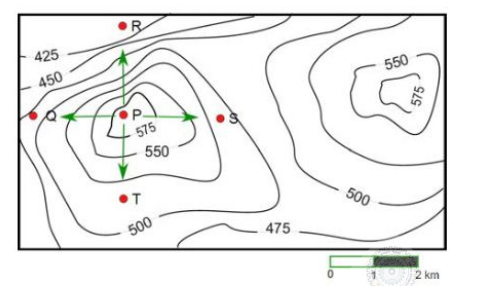
\includegraphics[width=0.5\columnwidth]{Figs/fig1.png}
    \caption{Q.65}
    \label{fig:q65}
\end{figure}
Which of the following is the steepest path leaving from P?
\begin{enumerate}
\begin{multicols}{2}
\item P to Q
\item P to R
\item P to S
\item P to T
\end{multicols}
\end{enumerate}
\hfill (GATE MA 2017)

\end{enumerate}
\end{document}